\documentclass{standalone}
\usepackage{tikz}
\usetikzlibrary{patterns, positioning}


\begin{document}
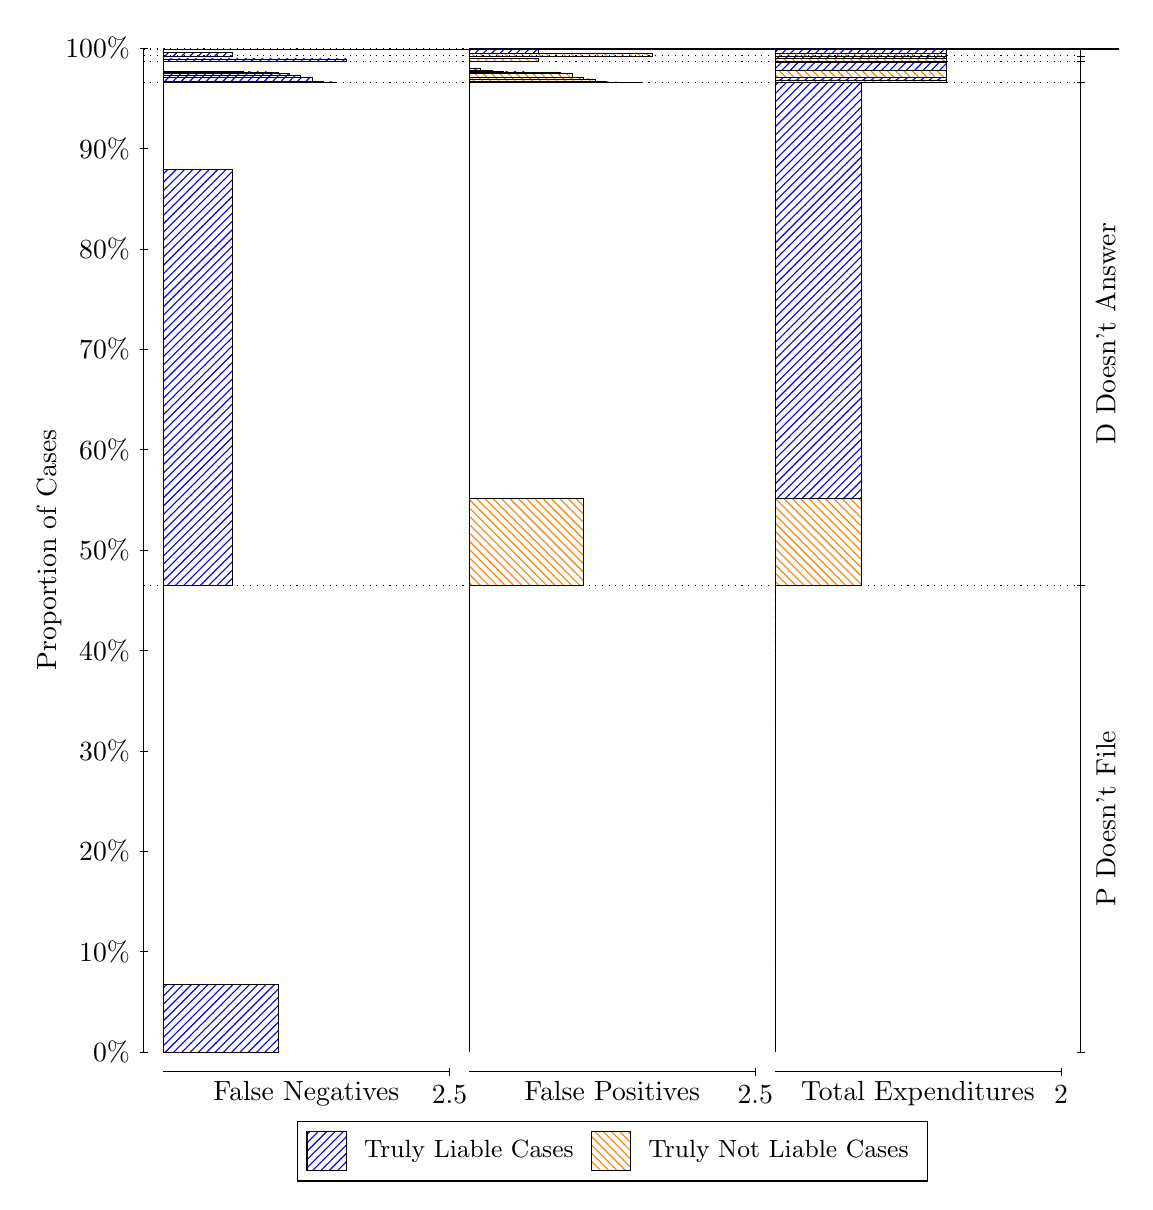
\begin{tikzpicture}
\draw[black, very thin] (1.5,1.75) -- (1.5,14.5);
\node[rotate=90, text=black, anchor=center] at (0.3, 8.125) {Proportion of Cases};
\draw[black, very thin] (1.45,1.75) -- (1.55,1.75);
\node[text=black, anchor=east] at (1.45, 1.75) {0\%};
\draw[black, very thin] (1.45,3.025) -- (1.55,3.025);
\node[text=black, anchor=east] at (1.45, 3.025) {10\%};
\draw[black, very thin] (1.45,4.3) -- (1.55,4.3);
\node[text=black, anchor=east] at (1.45, 4.3) {20\%};
\draw[black, very thin] (1.45,5.575) -- (1.55,5.575);
\node[text=black, anchor=east] at (1.45, 5.575) {30\%};
\draw[black, very thin] (1.45,6.85) -- (1.55,6.85);
\node[text=black, anchor=east] at (1.45, 6.85) {40\%};
\draw[black, very thin] (1.45,8.125) -- (1.55,8.125);
\node[text=black, anchor=east] at (1.45, 8.125) {50\%};
\draw[black, very thin] (1.45,9.4) -- (1.55,9.4);
\node[text=black, anchor=east] at (1.45, 9.4) {60\%};
\draw[black, very thin] (1.45,10.675) -- (1.55,10.675);
\node[text=black, anchor=east] at (1.45, 10.675) {70\%};
\draw[black, very thin] (1.45,11.95) -- (1.55,11.95);
\node[text=black, anchor=east] at (1.45, 11.95) {80\%};
\draw[black, very thin] (1.45,13.225) -- (1.55,13.225);
\node[text=black, anchor=east] at (1.45, 13.225) {90\%};
\draw[black, very thin] (1.45,14.5) -- (1.55,14.5);
\node[text=black, anchor=east] at (1.45, 14.5) {100\%};

\draw[black, very thin] (13.4,1.75) -- (13.4,14.5);
\draw[black, very thin] (13.35,1.75) -- (13.45,1.75);
\node[anchor=west] at (13.35, 1.75) {};
\draw[black, very thin] (13.35,7.6752) -- (13.45,7.6752);
\node[anchor=west] at (13.35, 7.6752) {};
\draw[black, very thin] (13.35,14.065) -- (13.45,14.065);
\node[anchor=west] at (13.35, 14.065) {};
\draw[black, very thin] (13.35,14.329) -- (13.45,14.329);
\node[anchor=west] at (13.35, 14.329) {};
\draw[black, very thin] (13.35,14.4) -- (13.45,14.4);
\node[anchor=west] at (13.35, 14.4) {};
\draw[black, very thin] (13.35,14.478) -- (13.45,14.478);
\node[anchor=west] at (13.35, 14.478) {};
\draw[black, very thin] (13.35,14.487) -- (13.45,14.487);
\node[anchor=west] at (13.35, 14.487) {};
\draw[black, very thin] (13.35,14.5) -- (13.45,14.5);
\node[anchor=west] at (13.35, 14.5) {};

\draw[black, very thin, pattern color=blue, pattern=north east lines] (1.75,1.75) rectangle (3.2033,2.6112);
\draw[black, very thin, pattern color=orange, pattern=north west lines] (1.75,2.6112) rectangle (1.75,7.6752);
\draw[black, very thin, pattern color=blue, pattern=north east lines] (1.75,7.6752) rectangle (2.622,12.962);
\draw[black, very thin, pattern color=orange, pattern=north west lines] (1.75,12.962) rectangle (1.75,14.065);
\draw[black, very thin, pattern color=blue, pattern=north east lines] (1.75,14.065) rectangle (3.93,14.069);
\draw[black, very thin, pattern color=blue, pattern=north east lines] (1.75,14.069) rectangle (3.7847,14.081);
\draw[black, very thin, pattern color=blue, pattern=north east lines] (1.75,14.081) rectangle (3.6393,14.125);
\draw[black, very thin, pattern color=blue, pattern=north east lines] (1.75,14.125) rectangle (3.494,14.15);
\draw[black, very thin, pattern color=blue, pattern=north east lines] (1.75,14.15) rectangle (3.3487,14.18);
\draw[black, very thin, pattern color=blue, pattern=north east lines] (1.75,14.18) rectangle (3.2033,14.189);
\draw[black, very thin, pattern color=blue, pattern=north east lines] (1.75,14.189) rectangle (3.058,14.196);
\draw[black, very thin, pattern color=blue, pattern=north east lines] (1.75,14.196) rectangle (2.9127,14.198);
\draw[black, very thin, pattern color=blue, pattern=north east lines] (1.75,14.198) rectangle (2.7673,14.201);
\draw[black, very thin, pattern color=orange, pattern=north west lines] (1.75,14.201) rectangle (1.75,14.329);
\draw[black, very thin, pattern color=blue, pattern=north east lines] (1.75,14.329) rectangle (4.0753,14.362);
\draw[black, very thin, pattern color=orange, pattern=north west lines] (1.75,14.362) rectangle (1.75,14.4);
\draw[black, very thin, pattern color=blue, pattern=north east lines] (1.75,14.4) rectangle (2.622,14.446);
\draw[black, very thin, pattern color=orange, pattern=north west lines] (1.75,14.446) rectangle (1.75,14.478);
\draw[black, very thin, pattern color=blue, pattern=north east lines] (1.75,14.478) rectangle (6.6913,14.481);
\draw[black, very thin, pattern color=orange, pattern=north west lines] (1.75,14.481) rectangle (1.75,14.487);
\draw[black, very thin, pattern color=orange, pattern=north west lines] (1.75,14.487) rectangle (1.75,14.491);
\draw[black, very thin, pattern color=blue, pattern=north east lines] (1.75,14.491) rectangle (1.75,14.5);
\draw[black, very thin, pattern color=orange, pattern=north west lines] (5.6333,1.75) rectangle (5.6333,6.8139);
\draw[black, very thin, pattern color=blue, pattern=north east lines] (5.6333,6.8139) rectangle (5.6333,7.6752);
\draw[black, very thin, pattern color=orange, pattern=north west lines] (5.6333,7.6752) rectangle (7.0867,8.7785);
\draw[black, very thin, pattern color=blue, pattern=north east lines] (5.6333,8.7785) rectangle (5.6333,14.065);
\draw[black, very thin, pattern color=orange, pattern=north west lines] (5.6333,14.065) rectangle (7.8133,14.066);
\draw[black, very thin, pattern color=orange, pattern=north west lines] (5.6333,14.066) rectangle (7.668,14.067);
\draw[black, very thin, pattern color=orange, pattern=north west lines] (5.6333,14.067) rectangle (7.5227,14.071);
\draw[black, very thin, pattern color=orange, pattern=north west lines] (5.6333,14.071) rectangle (7.3773,14.079);
\draw[black, very thin, pattern color=orange, pattern=north west lines] (5.6333,14.079) rectangle (7.232,14.108);
\draw[black, very thin, pattern color=orange, pattern=north west lines] (5.6333,14.108) rectangle (7.0867,14.132);
\draw[black, very thin, pattern color=orange, pattern=north west lines] (5.6333,14.132) rectangle (6.9413,14.176);
\draw[black, very thin, pattern color=orange, pattern=north west lines] (5.6333,14.176) rectangle (6.796,14.188);
\draw[black, very thin, pattern color=orange, pattern=north west lines] (5.6333,14.188) rectangle (6.6507,14.193);
\draw[black, very thin, pattern color=blue, pattern=north east lines] (5.6333,14.193) rectangle (6.36,14.196);
\draw[black, very thin, pattern color=blue, pattern=north east lines] (5.6333,14.196) rectangle (6.2147,14.198);
\draw[black, very thin, pattern color=blue, pattern=north east lines] (5.6333,14.198) rectangle (6.0693,14.205);
\draw[black, very thin, pattern color=blue, pattern=north east lines] (5.6333,14.205) rectangle (5.924,14.214);
\draw[black, very thin, pattern color=blue, pattern=north east lines] (5.6333,14.214) rectangle (5.7787,14.245);
\draw[black, very thin, pattern color=blue, pattern=north east lines] (5.6333,14.245) rectangle (5.6333,14.329);
\draw[black, very thin, pattern color=orange, pattern=north west lines] (5.6333,14.329) rectangle (6.5053,14.367);
\draw[black, very thin, pattern color=blue, pattern=north east lines] (5.6333,14.367) rectangle (5.6333,14.4);
\draw[black, very thin, pattern color=orange, pattern=north west lines] (5.6333,14.4) rectangle (7.9587,14.432);
\draw[black, very thin, pattern color=blue, pattern=north east lines] (5.6333,14.432) rectangle (6.5053,14.478);
\draw[black, very thin, pattern color=orange, pattern=north west lines] (5.6333,14.478) rectangle (5.6333,14.485);
\draw[black, very thin, pattern color=blue, pattern=north east lines] (5.6333,14.485) rectangle (5.6333,14.487);
\draw[black, very thin, pattern color=orange, pattern=north west lines] (5.6333,14.487) rectangle (10.575,14.491);
\draw[black, very thin, pattern color=blue, pattern=north east lines] (5.6333,14.491) rectangle (9.1213,14.5);
\draw[black, very thin, pattern color=orange, pattern=north west lines] (9.5167,1.75) rectangle (9.5167,6.8139);
\draw[black, very thin, pattern color=blue, pattern=north east lines] (9.5167,6.8139) rectangle (9.5167,7.6752);
\draw[black, very thin, pattern color=orange, pattern=north west lines] (9.5167,7.6752) rectangle (10.607,8.7785);
\draw[black, very thin, pattern color=blue, pattern=north east lines] (9.5167,8.7785) rectangle (10.607,14.065);
\draw[black, very thin, pattern color=orange, pattern=north west lines] (9.5167,14.065) rectangle (11.697,14.094);
\draw[black, very thin, pattern color=blue, pattern=north east lines] (9.5167,14.094) rectangle (11.697,14.124);
\draw[black, very thin, pattern color=orange, pattern=north west lines] (9.5167,14.124) rectangle (11.697,14.218);
\draw[black, very thin, pattern color=blue, pattern=north east lines] (9.5167,14.218) rectangle (11.697,14.314);
\draw[black, very thin, pattern color=orange, pattern=north west lines] (9.5167,14.314) rectangle (11.697,14.32);
\draw[black, very thin, pattern color=blue, pattern=north east lines] (9.5167,14.32) rectangle (11.697,14.329);
\draw[black, very thin, pattern color=orange, pattern=north west lines] (9.5167,14.329) rectangle (11.697,14.367);
\draw[black, very thin, pattern color=blue, pattern=north east lines] (9.5167,14.367) rectangle (11.697,14.4);
\draw[black, very thin, pattern color=orange, pattern=north west lines] (9.5167,14.4) rectangle (11.697,14.432);
\draw[black, very thin, pattern color=blue, pattern=north east lines] (9.5167,14.432) rectangle (11.697,14.478);
\draw[black, very thin, pattern color=orange, pattern=north west lines] (9.5167,14.478) rectangle (13.877,14.485);
\draw[black, very thin, pattern color=blue, pattern=north east lines] (9.5167,14.485) rectangle (13.877,14.487);
\draw[black, very thin, pattern color=orange, pattern=north west lines] (9.5167,14.487) rectangle (13.877,14.491);
\draw[black, very thin, pattern color=blue, pattern=north east lines] (9.5167,14.491) rectangle (13.877,14.5);
\draw[black, dotted] (1.5,7.6752) -- (13.4,7.6752);
\draw[black, dotted] (1.5,14.065) -- (13.4,14.065);
\draw[black, dotted] (1.5,14.329) -- (13.4,14.329);
\draw[black, dotted] (1.5,14.4) -- (13.4,14.4);
\draw[black, dotted] (1.5,14.478) -- (13.4,14.478);
\draw[black, dotted] (1.5,14.487) -- (13.4,14.487);
\draw[black, very thin] (1.75,1.5) -- (5.3833,1.5);
\node[text=black, anchor=north] at (3.5667, 1.5) {False Negatives};
\draw[black, very thin] (5.3833,1.45) -- (5.3833,1.55);
\node[text=black, anchor=north] at (5.3833, 1.45) {2.5};

\draw[black, very thin] (5.6333,1.5) -- (9.2667,1.5);
\node[text=black, anchor=north] at (7.45, 1.5) {False Positives};
\draw[black, very thin] (9.2667,1.45) -- (9.2667,1.55);
\node[text=black, anchor=north] at (9.2667, 1.45) {2.5};

\draw[black, very thin] (9.5167,1.5) -- (13.15,1.5);
\node[text=black, anchor=north] at (11.333, 1.5) {Total Expenditures};
\draw[black, very thin] (13.15,1.45) -- (13.15,1.55);
\node[text=black, anchor=north] at (13.15, 1.45) {2};

\node[text=black, centered, rotate=90] at (13.72, 4.7126) {P Doesn't File};
\node[text=black, centered, rotate=90] at (13.72, 10.87) {D Doesn't Answer};






\draw (7.449999999999999,1.5) node[draw=none] (baseCoordinate) {};
\begin{scope}[align=center]
        \matrix[scale=0.5, draw=black, below=0.5cm of baseCoordinate, nodes={draw}, column sep=0.1cm]{
            \node[rectangle, draw, minimum width=0.5cm, minimum height=0.5cm, pattern color=blue, pattern=north east lines] {}; &
            \node[draw=none, font=\small, text=black] (B) {Truly Liable Cases}; &
            \node[rectangle, draw, minimum width=0.5cm, minimum height=0.5cm, pattern color=orange, pattern=north west lines] {}; &
            \node[draw=none, font=\small, text=black] (B) {Truly Not Liable Cases}; \\
            };
\end{scope}

\end{tikzpicture}
\end{document}